A two-dimensional linear system is a system of the form
\begin{equation}
	\begin{aligned}
		\dot{x}=ax+by\\
		\dot{y}=cx+dy
	\end{aligned}
\end{equation}
where $a$, $b$, $c$, $d$ are parameters.
If we use \textbf{boldface} to denote vectors, this system can be written more compactly in matrix form as
\begin{equation}{\label{eq:g2de}}
	\mathbf{\dot{x}}=A\mathbf{x} \quad \text{where} \quad 
	A=
	\begin{pmatrix}
		a&b\\c&d
	\end{pmatrix}\quad\text{and}\quad
	\mathbf{x}=
	\begin{pmatrix}
		x\\y
	\end{pmatrix}\quad
	\mathbf{\tilde{x}}=
	\begin{pmatrix}
		0\\0
	\end{pmatrix}
\end{equation} 
Notice that $\mathbf{\dot{x}}=0$ when $\mathbf{x}=0$, so $\mathbf{\tilde{x}}$ is always a fixed point for any choice of $A$.
The solutions of $\mathbf{\dot{x}}=A\mathbf{x}$ can be visualized as trajectories moving on the $(x,y)$ plane, in this context called the {\textbf{phase plane}}.\\\\
If the off-diagonal terms in (\ref{eq:g2de}), $b$ and $c$ are zero, we would have two seperate uncoupled equations in $x$ and $y$ (Equation (\ref{eq:c2de})).
Such kind of systems are called \textbf{Uncoupled Systems}.
However, there would be two special lines, where the trajectories starting on it would always stick to it, these are  $x$ and $y$ axes\label{txt:xya}.\\
Suppose $d=-1$, then the system has solution as shown in Figure (\ref{fig:cnls}).
\begin{equation}{\label{eq:c2de}}
	\begin{aligned}
		\dot{x}=ax\\
		\dot{y}=dy
	\end{aligned}\quad\rightarrow\quad
	\begin{aligned}
		A=\begin{pmatrix}
		a&0\\0&d
		\end{pmatrix}
	\end{aligned}\quad\rightarrow\quad
	\begin{aligned} 
		x(t)=x_0e^{at}\\
		y(t)=y_0e^{dt}
	\end{aligned}
\end{equation}
\begin{figure}[h!]
	\centering
	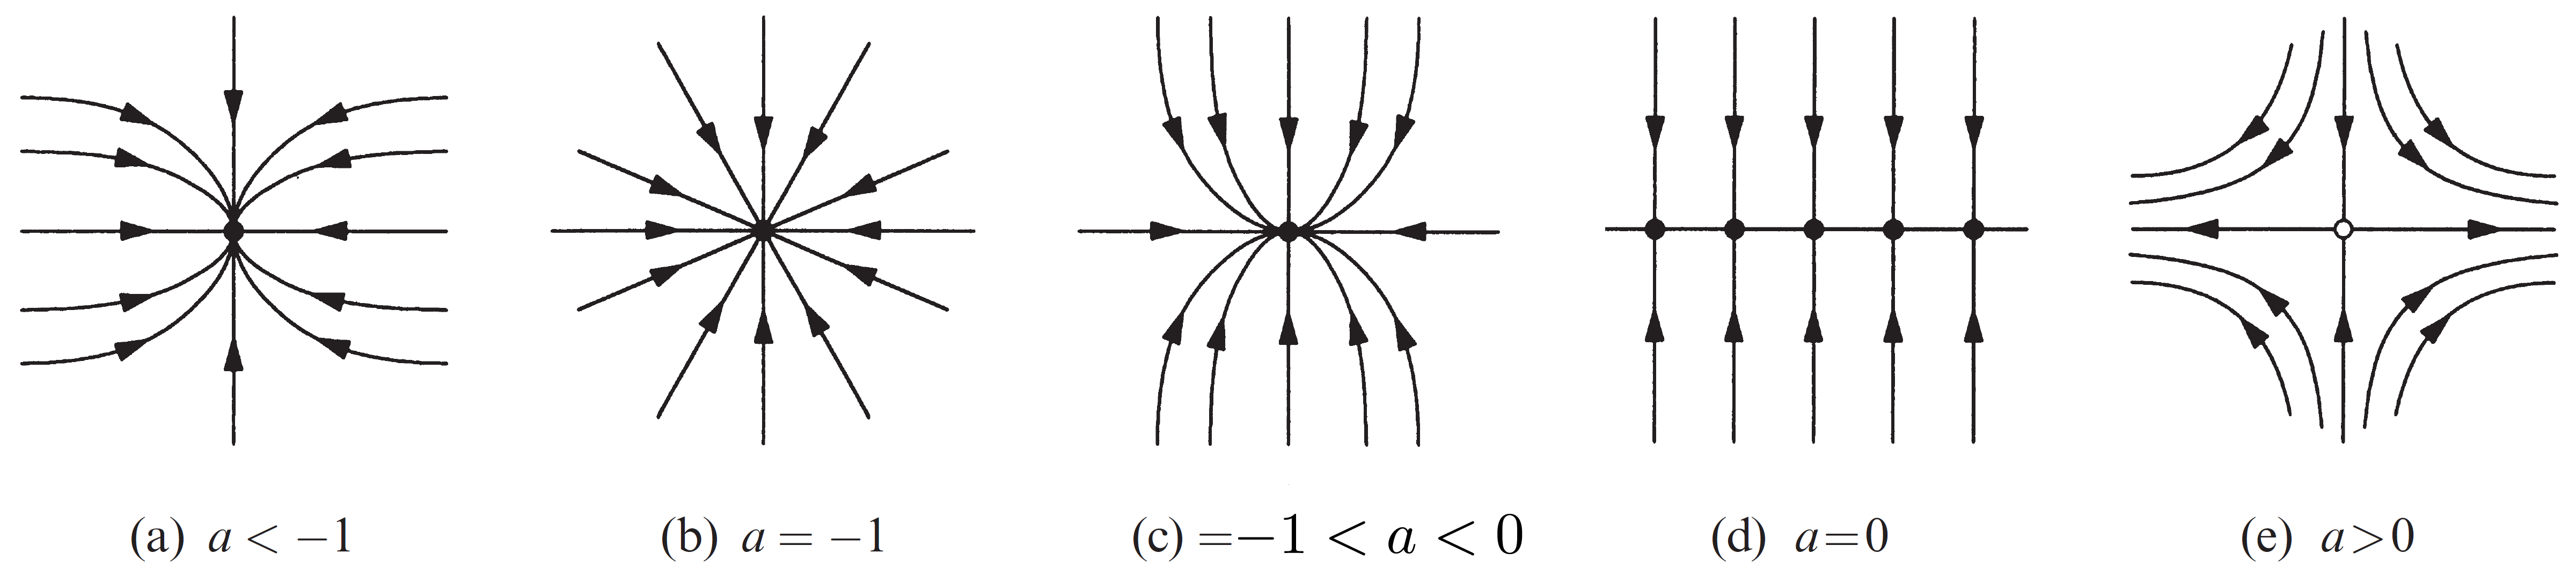
\includegraphics[width=0.9\linewidth]{cnls.png}
	\caption{Phase Portrait of Equation (\ref{eq:c2de}). See Section (\ref{sec:cls}) for classification.}
	\label{fig:cnls}
\end{figure}
\subsection{Classification of Two-Dimensional Linear Systems}{\label{sec:cls}}
There is the possibility of special lines (like $x$ and $y$ axis in case of uncoupled systems) existing for a general linear system having a matrix $A$.
The equation for finding such a direction is
\begin{equation}
	A\mathbf{x}=\lambda\mathbf{x}
\end{equation}
This is precisely the form of the eigenvalue problem whose solution is well known in the domain of linear algebra.
The eigenvalues of $A$ can be readily calculated and it is most convenient to express them in terms of the trace $(t_r)$ and determinant $(d_{et})$ of $A$.
\begin{equation}
	\begin{vmatrix}
		a-\lambda&b\\c&d-\lambda
	\end{vmatrix}
	=\lambda^2-\lambda\underbrace{(a+d)}_{t_r}+\underbrace{ad-bc}_{d_{et}}=0
\end{equation}
\begin{equation}
	\Rightarrow \lambda_{1,2}=\frac{1}{2}\{t_r\pm\sqrt{t_r^2-4d_{et}}\}
\end{equation}
The trace and determinant are invariant when the matrix $A$ is expressed by its eigenvalues and becomes diagonal
\begin{equation}
	A=
	\begin{pmatrix}
		\lambda_1&0\\0&\lambda_2
	\end{pmatrix}
	\quad \text{as} \quad
	\begin{aligned}
		\lambda_1+\lambda_2&=t_r\\
		\lambda_1\lambda_2&=d_{et}
	\end{aligned}
\end{equation}
\begin{enumerate}[label=\textbf{(\Alph*)}]
	\item Eigenvalues are Real
		\begin{equation}
			t_r^2-4d_{et}\geq0 \quad\rightarrow\quad \lambda_{1,2}\in\mathbb{R}
		\end{equation}
		\begin{enumerate}
			\item[\textbf{Case: (1.a)}]  $\lambda_1<\lambda_2<0$\quad|\quad\fbox{
	  			\mbox{$t_r^2-4d_{et}>0\quad d_{et}>0\quad t_r<0$}}\\
				This case is called a {\textbf{stable node}}, the only straight trajectories are along the eigendirections, which are given by the eigenvectors of the system.
				As $\lambda_1<\lambda_2$, the trajectories approach the fixed point faster along the direction of the eigenvector $\mathbf{v^{(1)}}$ which corresponds to $\lambda_1$, and is therefore called the \emph{fast eigendirection}.
				In the same way, the direction related to $\lambda_2$ is called the \emph{slow eigendirection}.
				\begin{figure}[h!]
					\centering
					\begin{subfigure}{0.4\linewidth}
						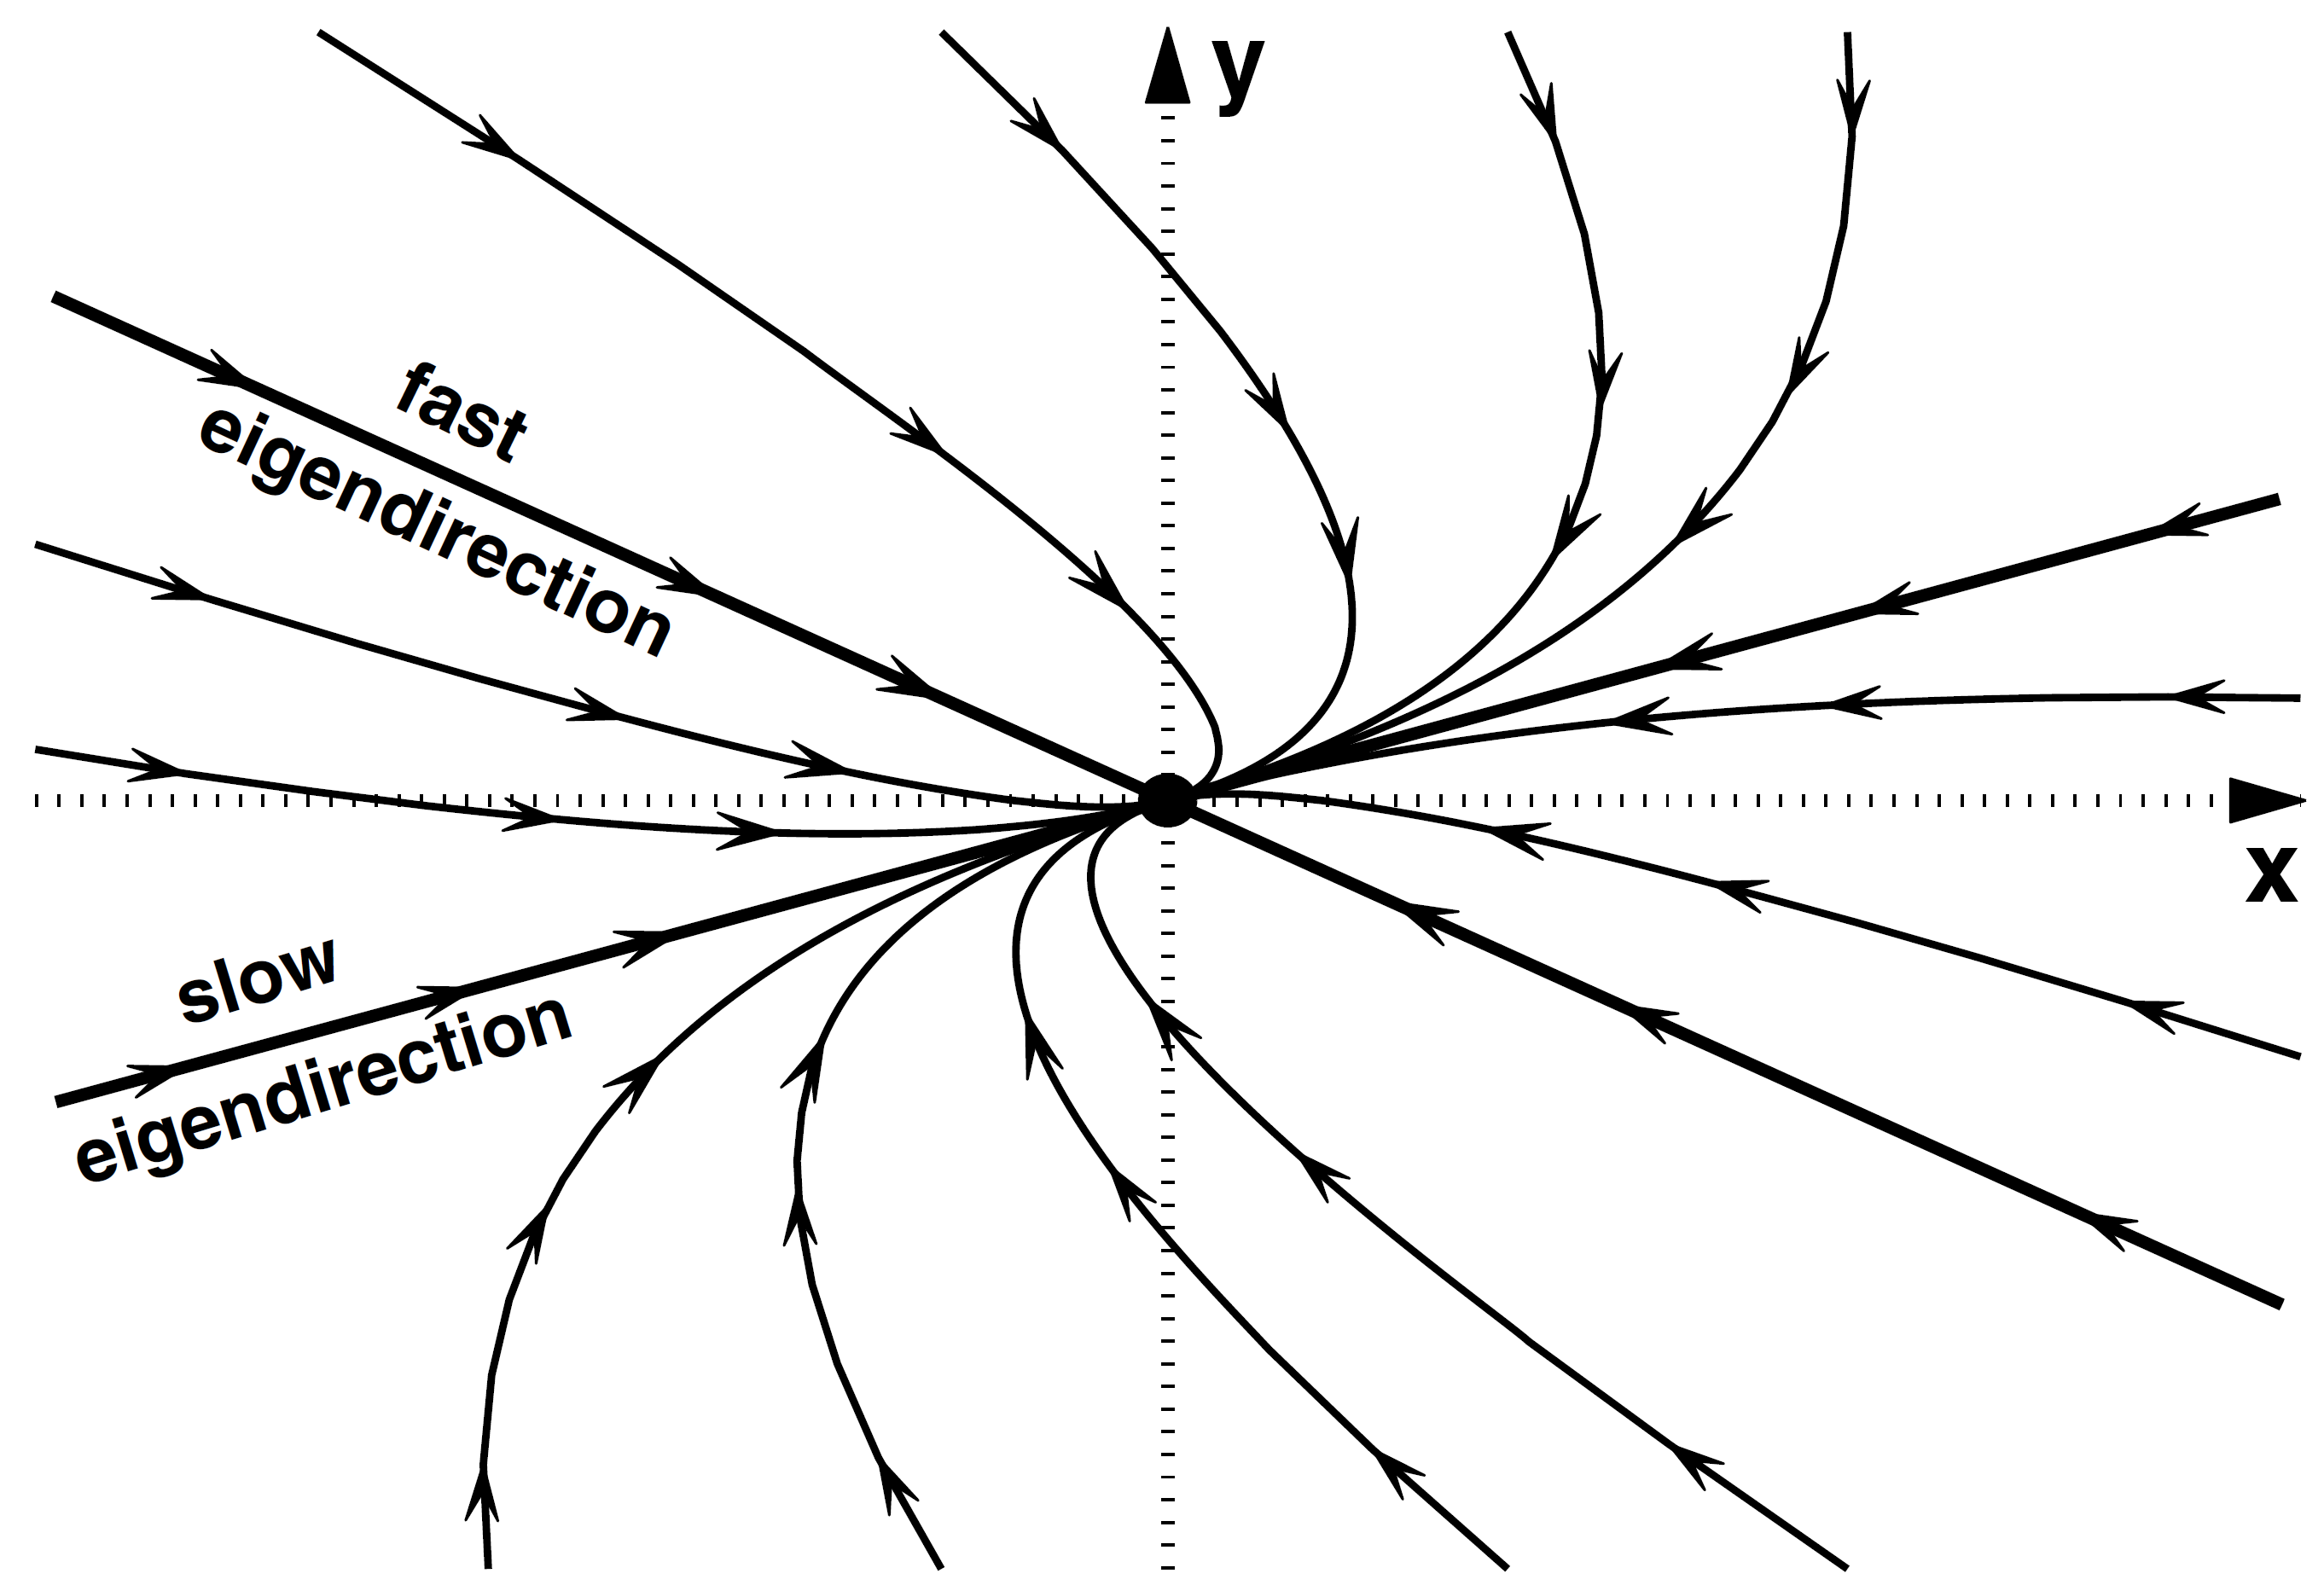
\includegraphics[width=\linewidth]{snls.png}
						\caption{Phase Portrait of a Stable Node}
						\label{fig:snls}
					\end{subfigure}
					\vline
					\begin{subfigure}{0.364\linewidth}
						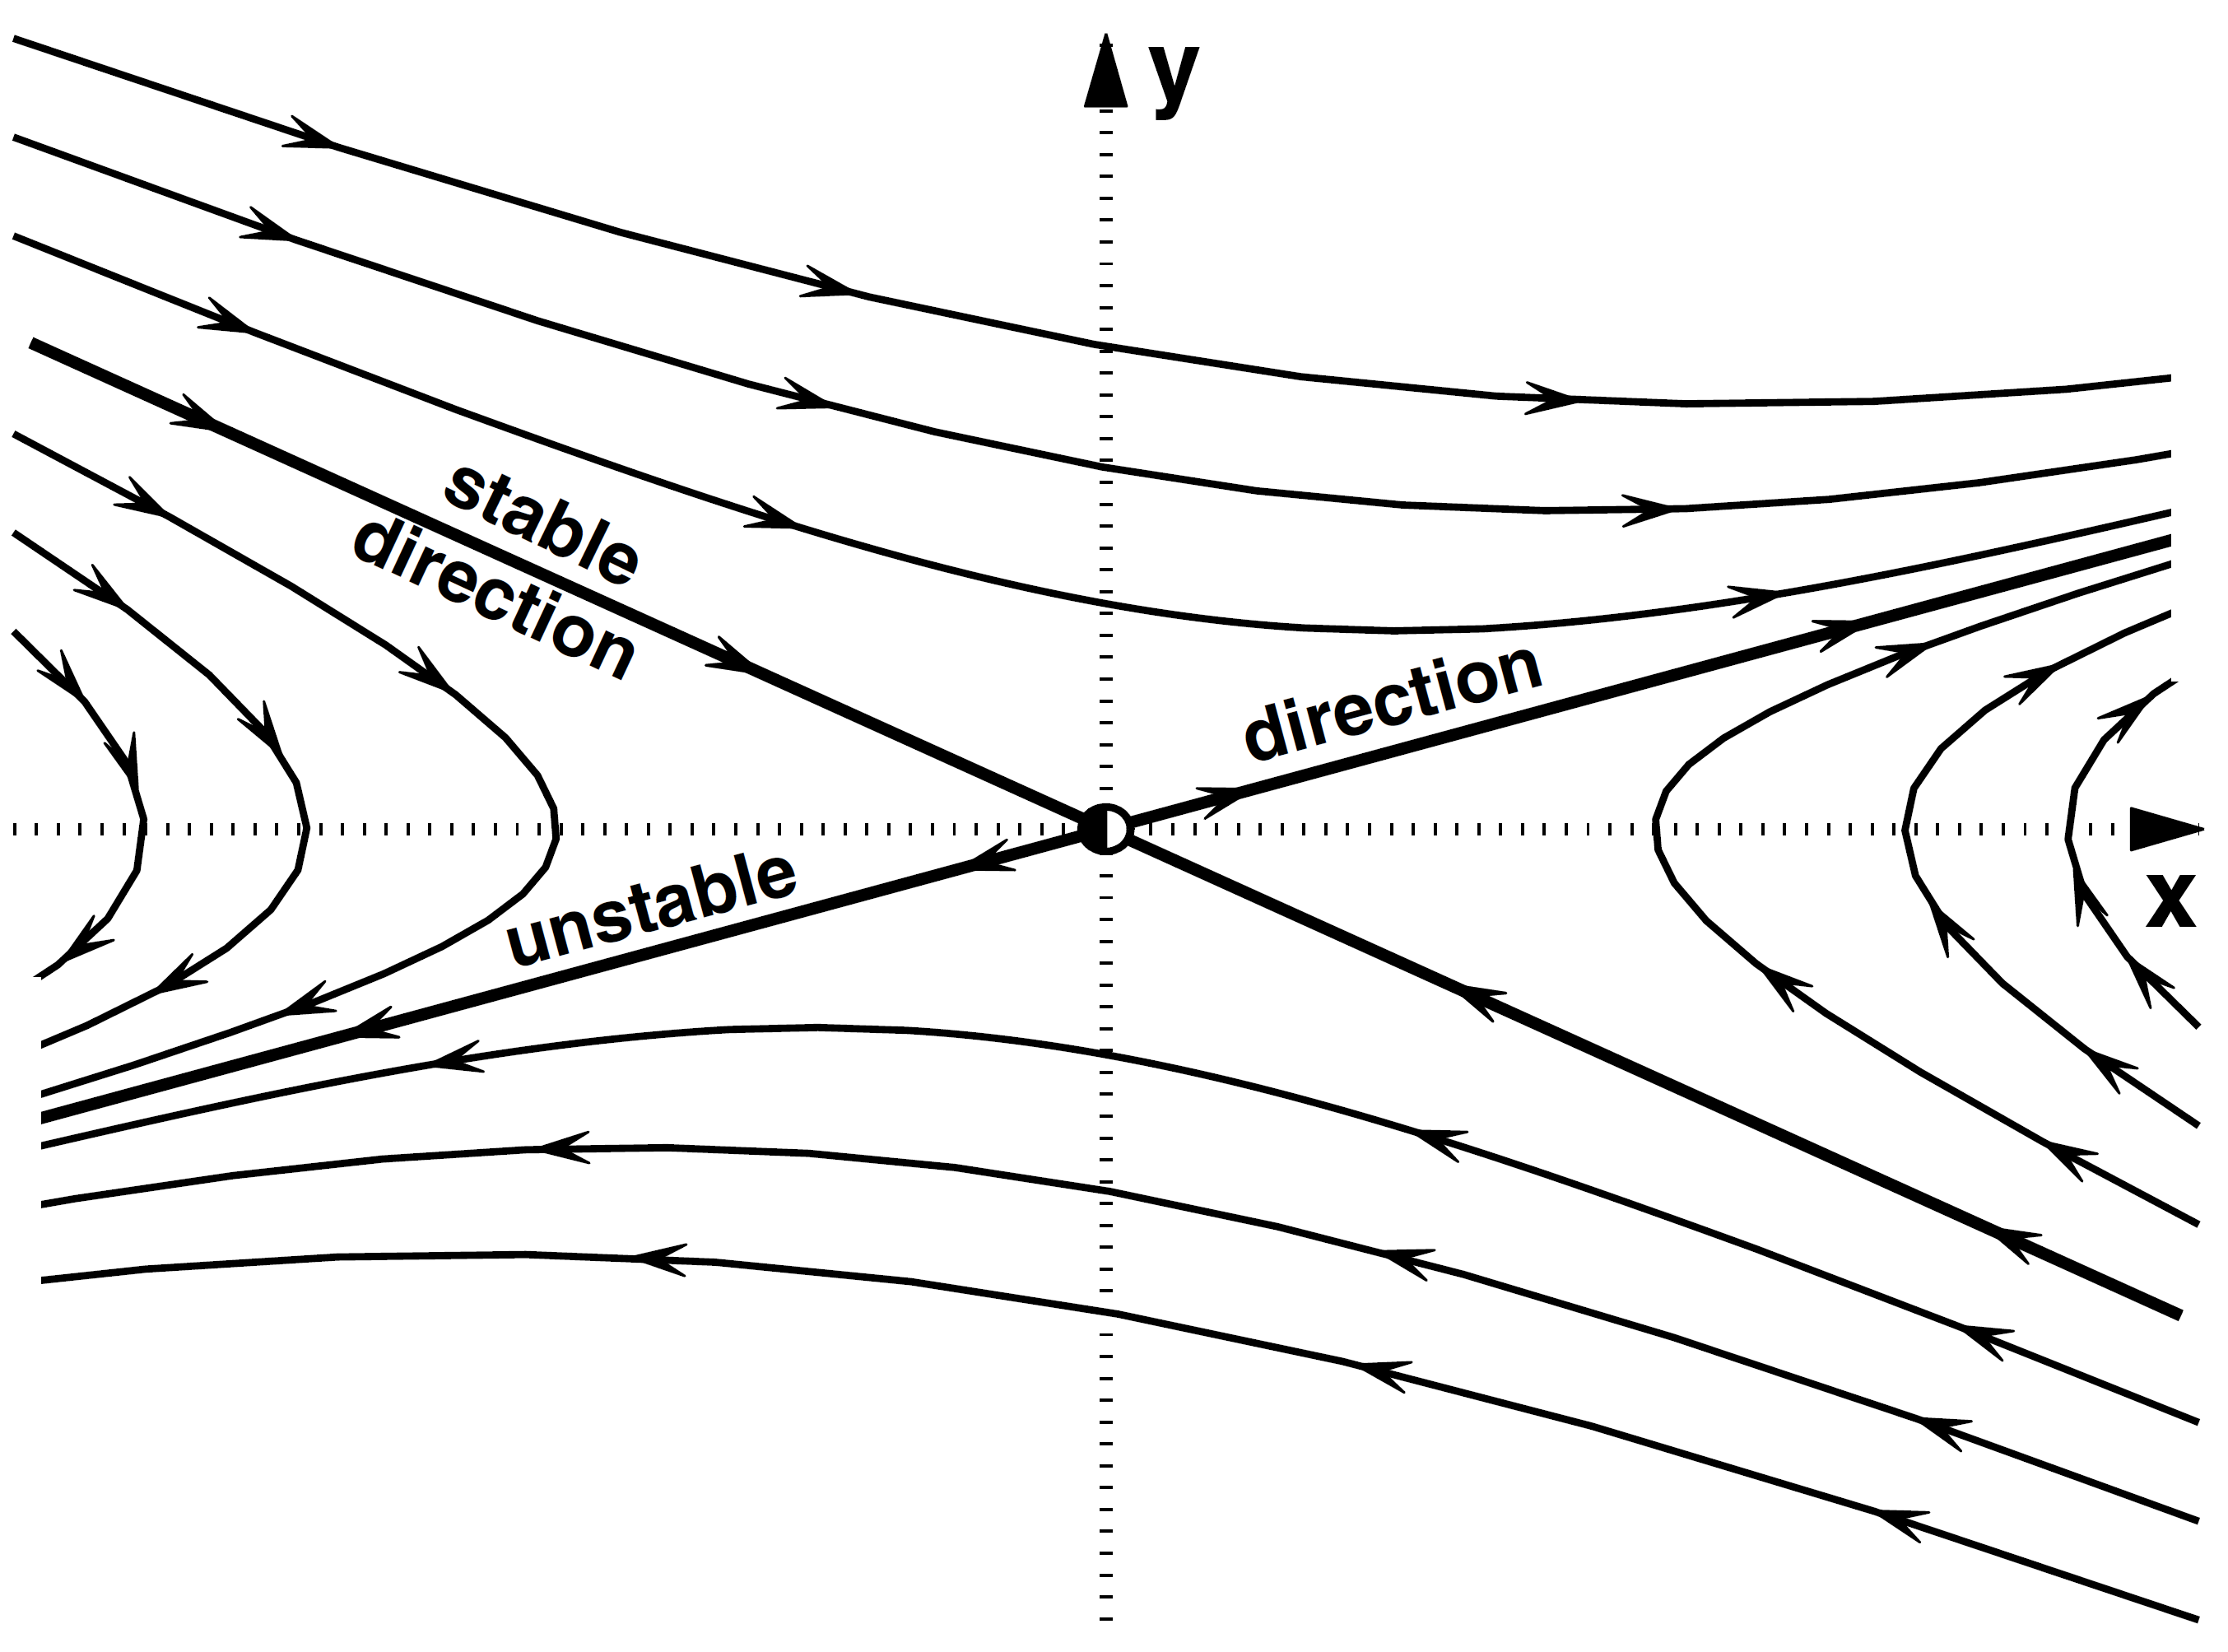
\includegraphics[width=\linewidth]{spls.png}
						\caption{Phase Portrait of a Saddle Point}
						\label{fig:spls}
					\end{subfigure}
					\caption{}
					\label{fig:cls1}
		    	\end{figure}
		    \item[\textbf{Case: (1.b)}] $0<\lambda_2<\lambda_1$\quad|\quad \fbox{
	  			\mbox{$t_r^2-4d_{et}>0\quad d_{et}>0\quad t_r>0$}}\\
		    	Correspondingly, for the phase space plot when both eigenvalues are positive, the flow, indicated by the arrows in Figure (\ref{fig:cls1}), is reversed and leads away from the fixed point, which is then called an {\textbf{unstable node}}.	    
		    \item[\textbf{Case: (2)}] $\lambda_1<0<\lambda_2$\quad|\quad \fbox{
	  			\mbox{$t_r^2-4d_{et}>0\quad d_{et}<0$}}\\
		    	If one of the eigenvalues is positive and the other negative, the fixed point at the origin is \emph{half-stable} and called a {\textbf{saddle point}}.
		    	The eigenvector that corresponds to the negative eigenvalue defines the direction where the flow in phase space is pointing towards the fixed point, the so-called {\textbf{stable manifold}} (stable direction), defined as the set of initial conditions $\mathbf{x}_0$ such that $\mathbf{x}(t)\rightarrow\mathbf{\tilde{x}}$ as $t\rightarrow\infty$.
		    	The positive eigenvalue is associated with the {\textbf{unstable manifold}} (unstable direction) which is set of initial conditions $\mathbf{x}_0$ such that $\mathbf{x}(t)\rightarrow\mathbf{\tilde{x}}$ as $t\rightarrow-\infty$.
		    	Here, the flow moves away from the fixed point\footnote{Note that a typical trajectory asymptotically approaches the unstable manifold as $t\rightarrow\infty$, and approaches the stable manifold as $t\rightarrow-\infty$.}. A typical phase space portrait is shown in Figure (\ref{fig:spls}).\\ \\	
		    	Now, let's see \emph{degenerate} cases
		    \item[\textbf{Case: (3.a)}] $\lambda_1=\lambda_2<0$\quad|\quad \fbox{
	  			\mbox{$t_r^2-4d_{et}=0\quad d_{et}>0\quad t_r<0$}}\\
		    	Let look at the system with
		    	\begin{equation}
			    	A=
			    	\begin{pmatrix}
				    	\lambda&b\\0&\lambda
			    	\end{pmatrix}\quad\rightarrow\quad \lambda_{1,2}=\lambda
		    	\end{equation}
		    	Then Eigenvectors are given by
		    	\begin{equation}
			    	\begin{pmatrix}
				    	\lambda&b\\0&\lambda
			    	\end{pmatrix}
			    	\begin{pmatrix}
				    	v_x\\v_y
			    	\end{pmatrix}=
			    	\lambda
			    	\begin{pmatrix}
				    	v_x\\v_y
			    	\end{pmatrix}
			    	\quad\rightarrow\quad
			    	\begin{aligned}
				    	\lambda v_x+bv_y&=\lambda v_x\\\lambda v_y&=\lambda v_y
			    	\end{aligned}
			    	\quad\rightarrow\quad
			    	bv_y=0
		    	\end{equation}
		    	\begin{enumerate}[label=(\roman*)]
			    	\item $b\neq0$\\
			    	The only eigendirection of $A$ is the horizontal axis with $v_y=0$. The fixed point is called a \emph{stable} {\textbf{degenerate node}} and its phase portrait shown in Figure (\ref{fig:stnls} left).
			    	\item $b=0$\\
			    	Any vector is an eigenvector and the trajectories are straight lines pointing towards the fixed point. The phase space portrait for this situation is shown in Figure (\ref{fig:stnls} right) and the fixed point is for obvious reasons called a \emph{stable} {\textbf{star node}}.
		    	\end{enumerate}
		    	\begin{figure}[h!]
					\centering
					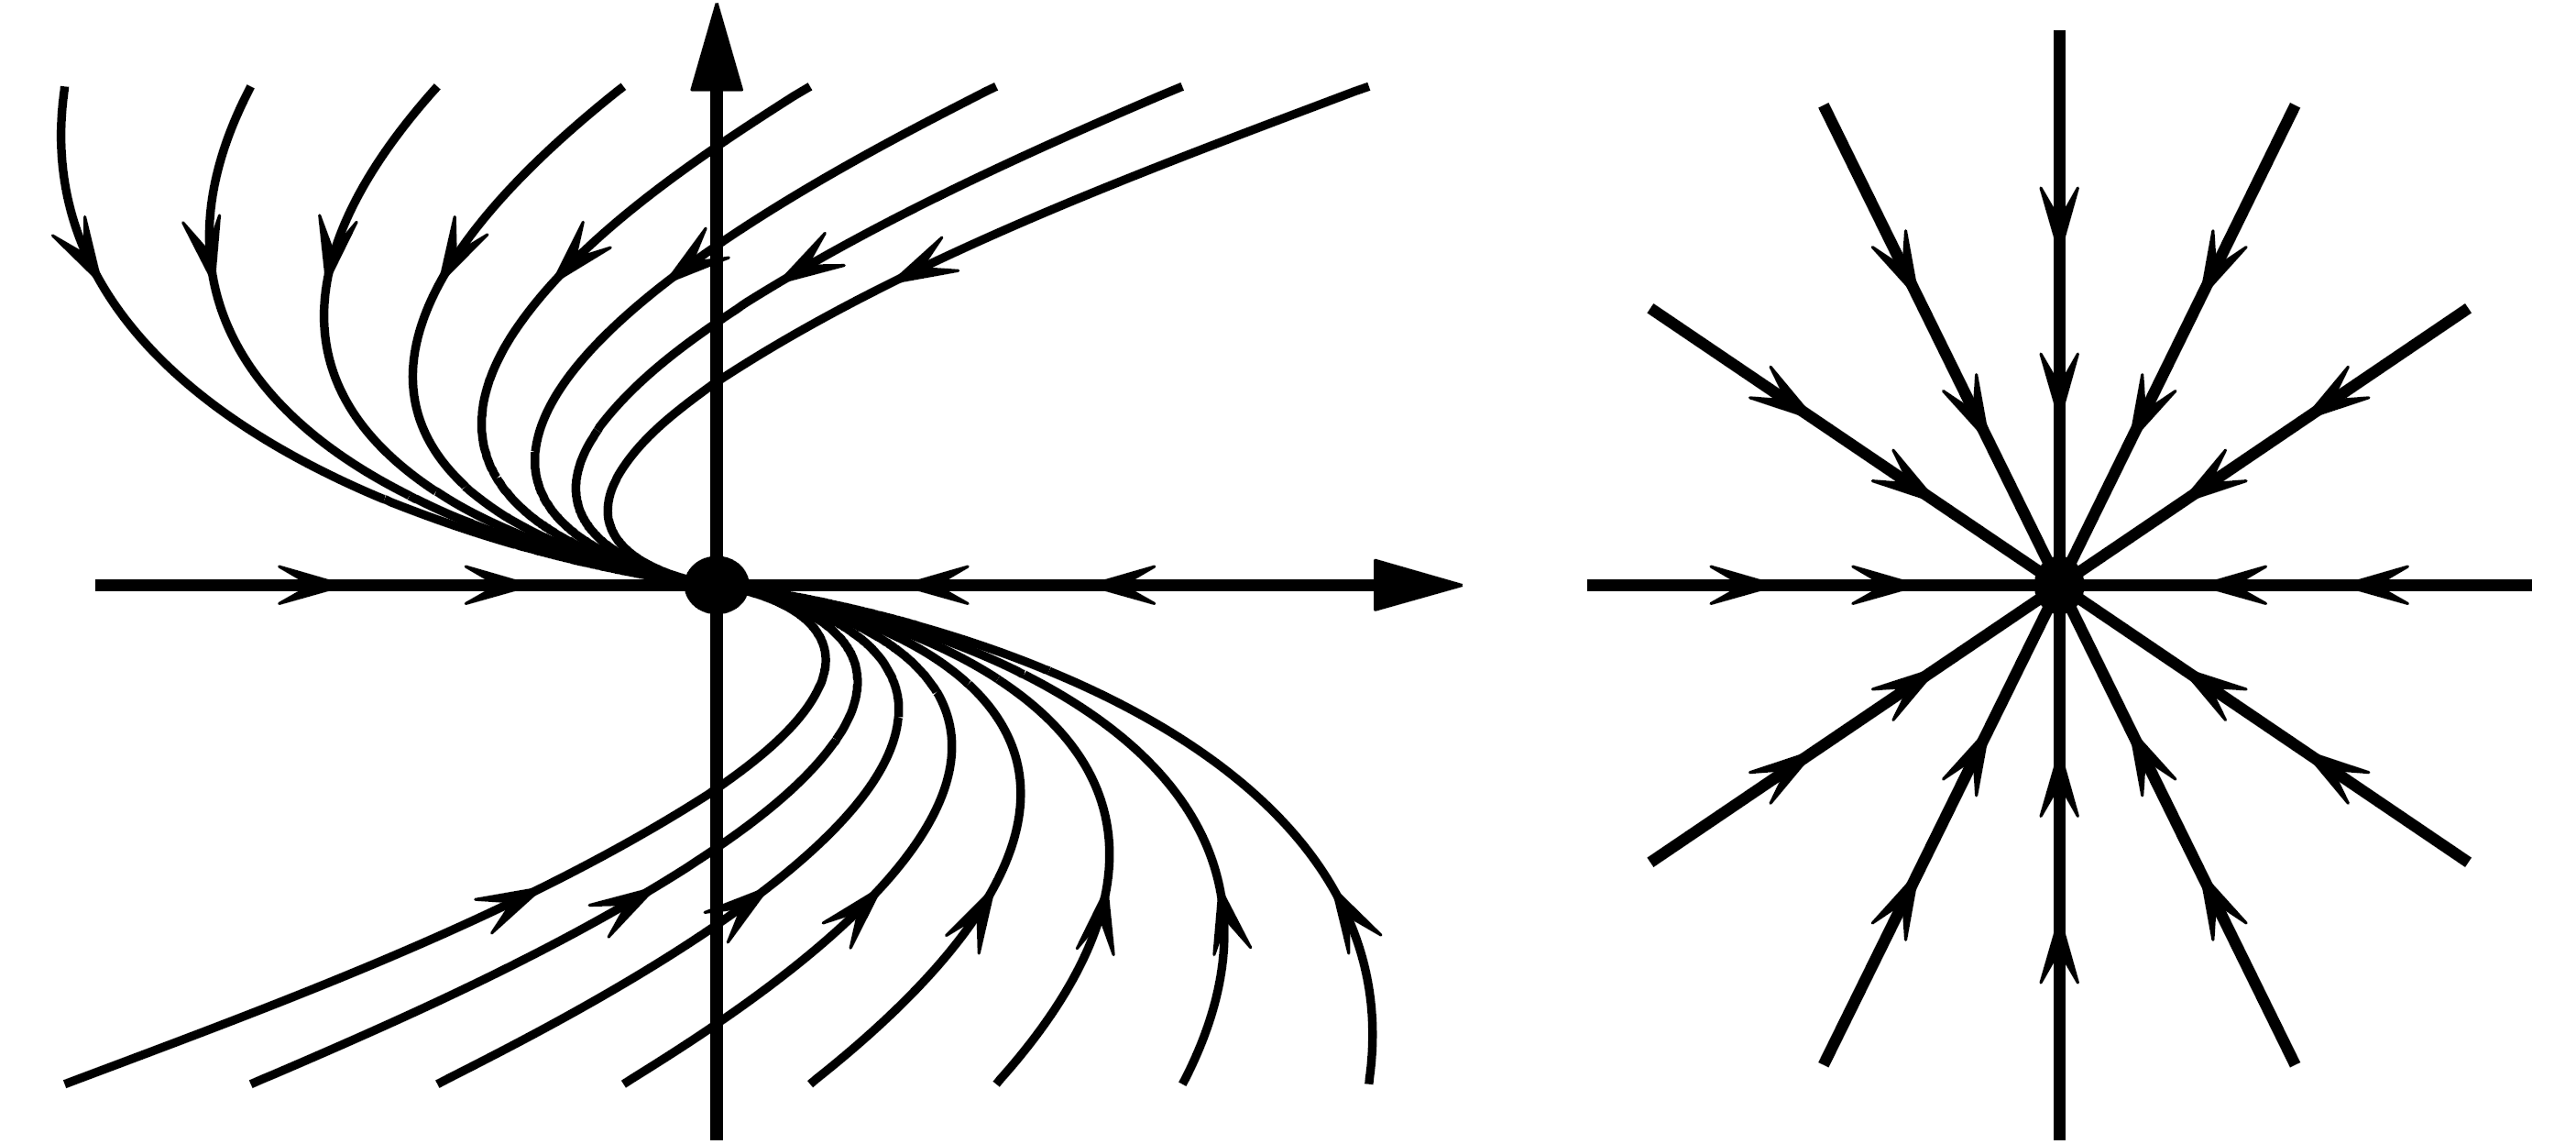
\includegraphics[width=0.6\linewidth]{dnls.png}
					\caption{Degenerate case where the eigenvalues are the same. The degenerate node (left) has only one eigendirection, the star node (right) has infinitely many.}
					\label{fig:stnls}
		    	\end{figure}
		    \item[\textbf{Case: (3.b)}] $\lambda_1=\lambda_2>0$\quad|\quad \fbox{
	  			\mbox{$t_r^2-4d_{et}=0\quad d_{et}>0\quad t_r>0$}}\\
		    	Similar as above
				\begin{enumerate}[label=(\roman*)]
			    	\item $b\neq0$\\
			    	The only eigendirection of $A$ is the horizontal axis with $v_y=0$.The flow, indicated by the arrows in Figure (\ref{fig:stnls} left), is reversed and leads away from the fixed point which is called a \emph{unstable} {\textbf{degenerate node}}.
			    	\item $b=0$\\
			    	Any vector is an eigenvector and the trajectories are straight lines pointing away from the fixed point.
			    	The flow, indicated by the arrows in Figure (\ref{fig:stnls} left), is reversed and the fixed point is for obvious reasons called a \emph{unstable} {\textbf{star node}}.
		    	\end{enumerate}	    
		    \item[\textbf{Case: (4.a)}] $\lambda_1<\lambda_2=0$\quad|\quad \fbox{
	  			\mbox{$t_r^2-4d_{et}>0\quad d_{et}=0\quad t_r<0$}}\\	
		    	Here, tragectories are parallel and towards a line of fixed points.
		    	The fixed point is {\textbf{Lyapunov stable}}\footnote{It means if all trajectories that start sufficiently close to $\mathbf{x}$ remain close to it for all time.} (Figure (\ref{fig:snils}) left).
		    \item[\textbf{Case: (4.b)}] $0=\lambda_1<\lambda_2$\quad|\quad \fbox{
	  			\mbox{$t_r^2-4d_{et}>0\quad d_{et}=0\quad t_r>0$}}\\
		    	Here, tragectories are parallel and towards a line of fixed points.
		    	These are \emph{unstable} {\textbf{non-isolated}} (Figure (\ref{fig:snils}) right).
				\begin{figure}[h!]
					\centering
					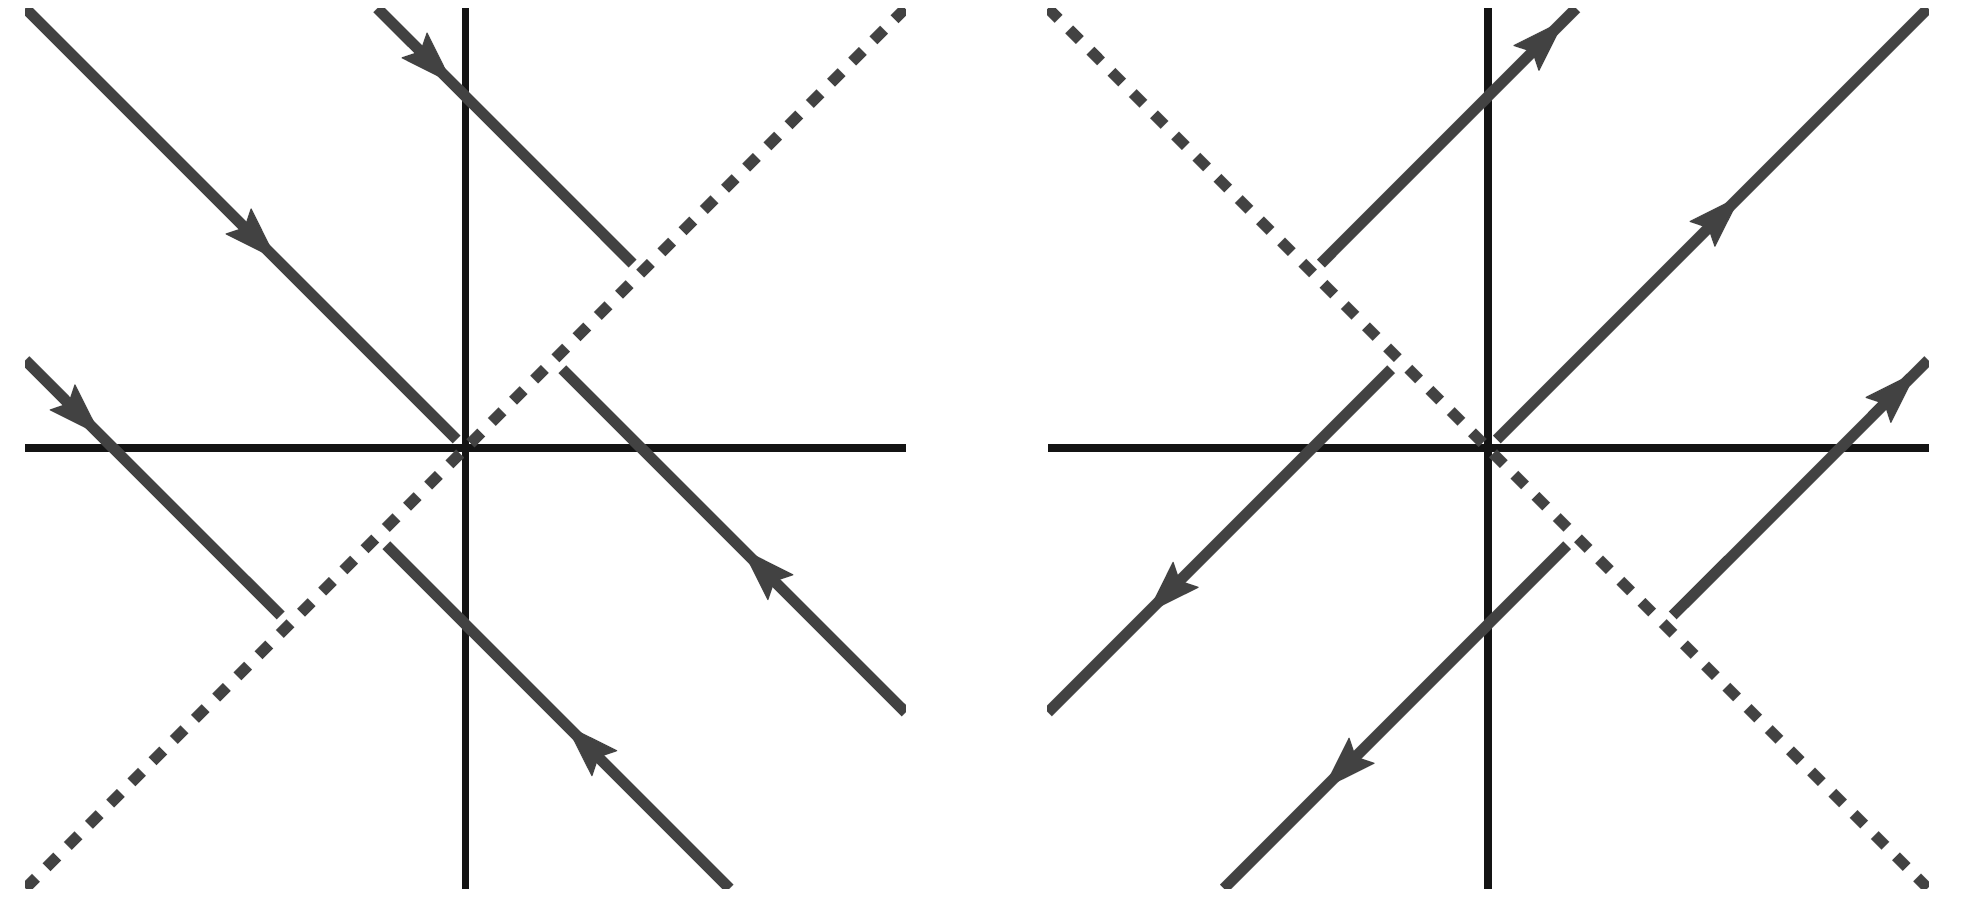
\includegraphics[width=0.4\linewidth]{snils.png}
					\caption{\emph{Stable non-isolated} fixed points on left and \emph{unstable non-isolated} fixed points on right }
					\label{fig:snils}
		    	\end{figure}
	    	\item[\textbf{Case: (5)}] $\lambda_1=\lambda_2=0$\quad|\quad \fbox{
	  			\mbox{$t_r^2-4d_{et}=0\quad d_{et}=0\quad t_r=0$}}\\
	    	Non-isolated fixed point, a plane of fixed points.
	    	Nothing happens and nothing can happen! Remember (\ref{eq:cons})?
		\end{enumerate}
	\item Eigenvalues are Complex (In fact, they are Complex Conjugate)
		\begin{equation}
			t_r^2-4d_{et}<0 \quad\rightarrow\quad \lambda_{1,2}\in\mathbb{C} \quad\rightarrow\quad \lambda_2=\lambda_1^\ast, \quad\text{Let} \ \Re(\lambda_{1,2})=\lambda\ \text{and}\ \Im(\lambda_{1,2})\neq0
		\end{equation}
		\begin{itemize}
			\item $\lambda<0$\quad|\quad \fbox{
	  		\mbox{$t_r^2-4d_{et}<0\quad d_{et}>0\quad t_r<0$}}\\
			The trajectories in phase space are spiraling towards from the origin as a {\textbf{stable spiral}} (Figure (\ref{fig:ccels}) left).
			\item $\lambda>0$\quad|\quad \fbox{
	  		\mbox{$t_r^2-4d_{et}<0\quad d_{et}>0\quad t_r>0$}}\\
			The trajectories in phase space are spiraling away from the origin as a {\textbf{unstable spiral}} (Figure (\ref{fig:ccels}) middle).
			\item $\lambda=0$\quad|\quad \fbox{
	  		\mbox{$t_r^2-4d_{et}<0\quad d_{et}>0\quad t_r=0$}}\\
			The trajectories are closed orbits.
			The fixed point $\tilde{x}=0$ is {\textbf{Lyapunov stable}}.
			The fixed point at the origin is neutrally stable and called a {\textbf{center}} (Figure (\ref{fig:ccels}) right).
			\begin{figure}[H]
				\centering
				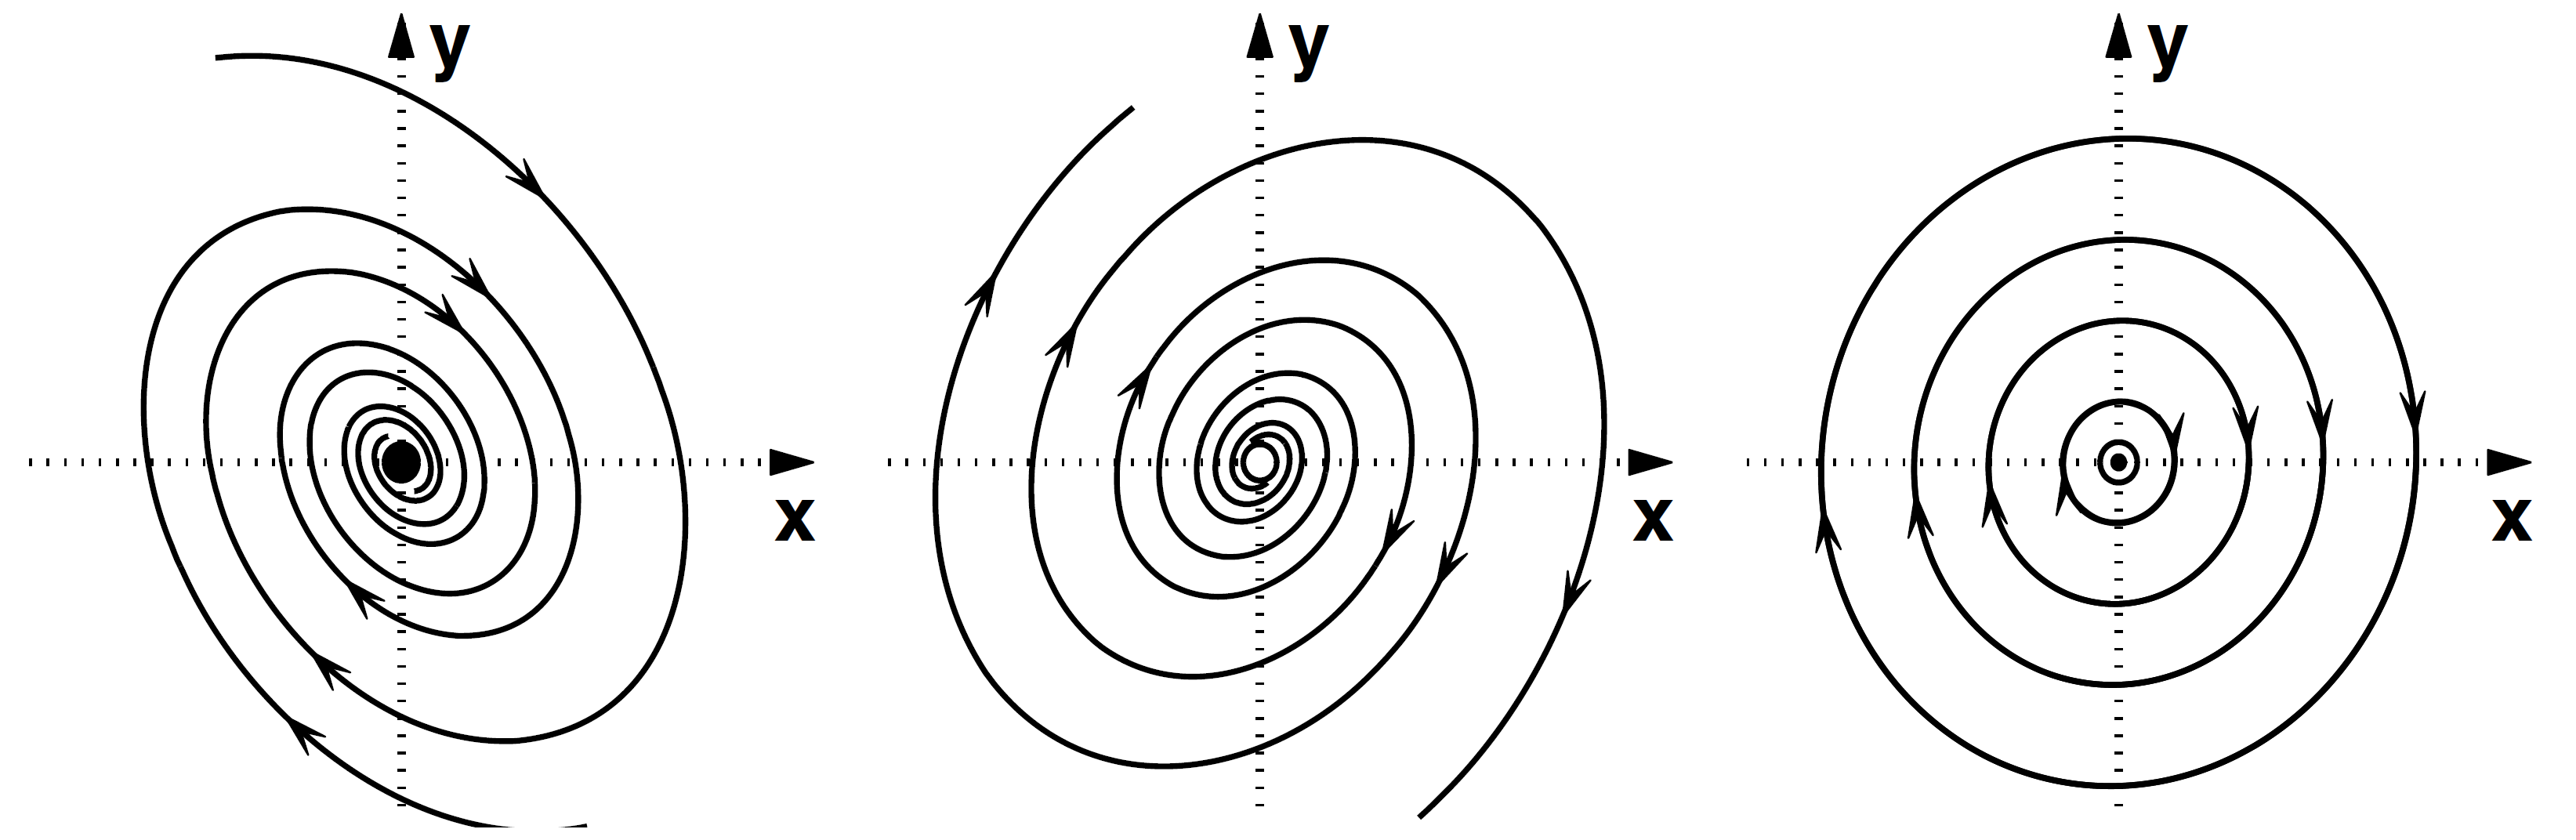
\includegraphics[width=0.5\linewidth]{ccels.png}
				\caption{For complex eigenvalues the trajectories in phase space are stable spirals if their real part is negative (left) and unstable spirals for a positive real part (middle). If the real part of the eigenvalues vanishes the trajectories are closed orbits around the origin, which is then a neutrally stable fixed point called a center (right).}
				\label{fig:ccels}
		    \end{figure}	
		\end{itemize}		
\end{enumerate}
\subsubsection{Summary}
On the left of the vertical axis $(d_{et}<0)$ are the saddle points.
On the right $(d_{et}>0)$ are the centers on the horizontal axis $(t_r=0)$ with unstable and stable spirals located above and below, respectively.
The stars and degenerate nodes exist along the parabola $t_r^2=4d_{et}$ that separates the spirals from the stable and unstable nodes.
\begin{figure}[h!]
	\centering
	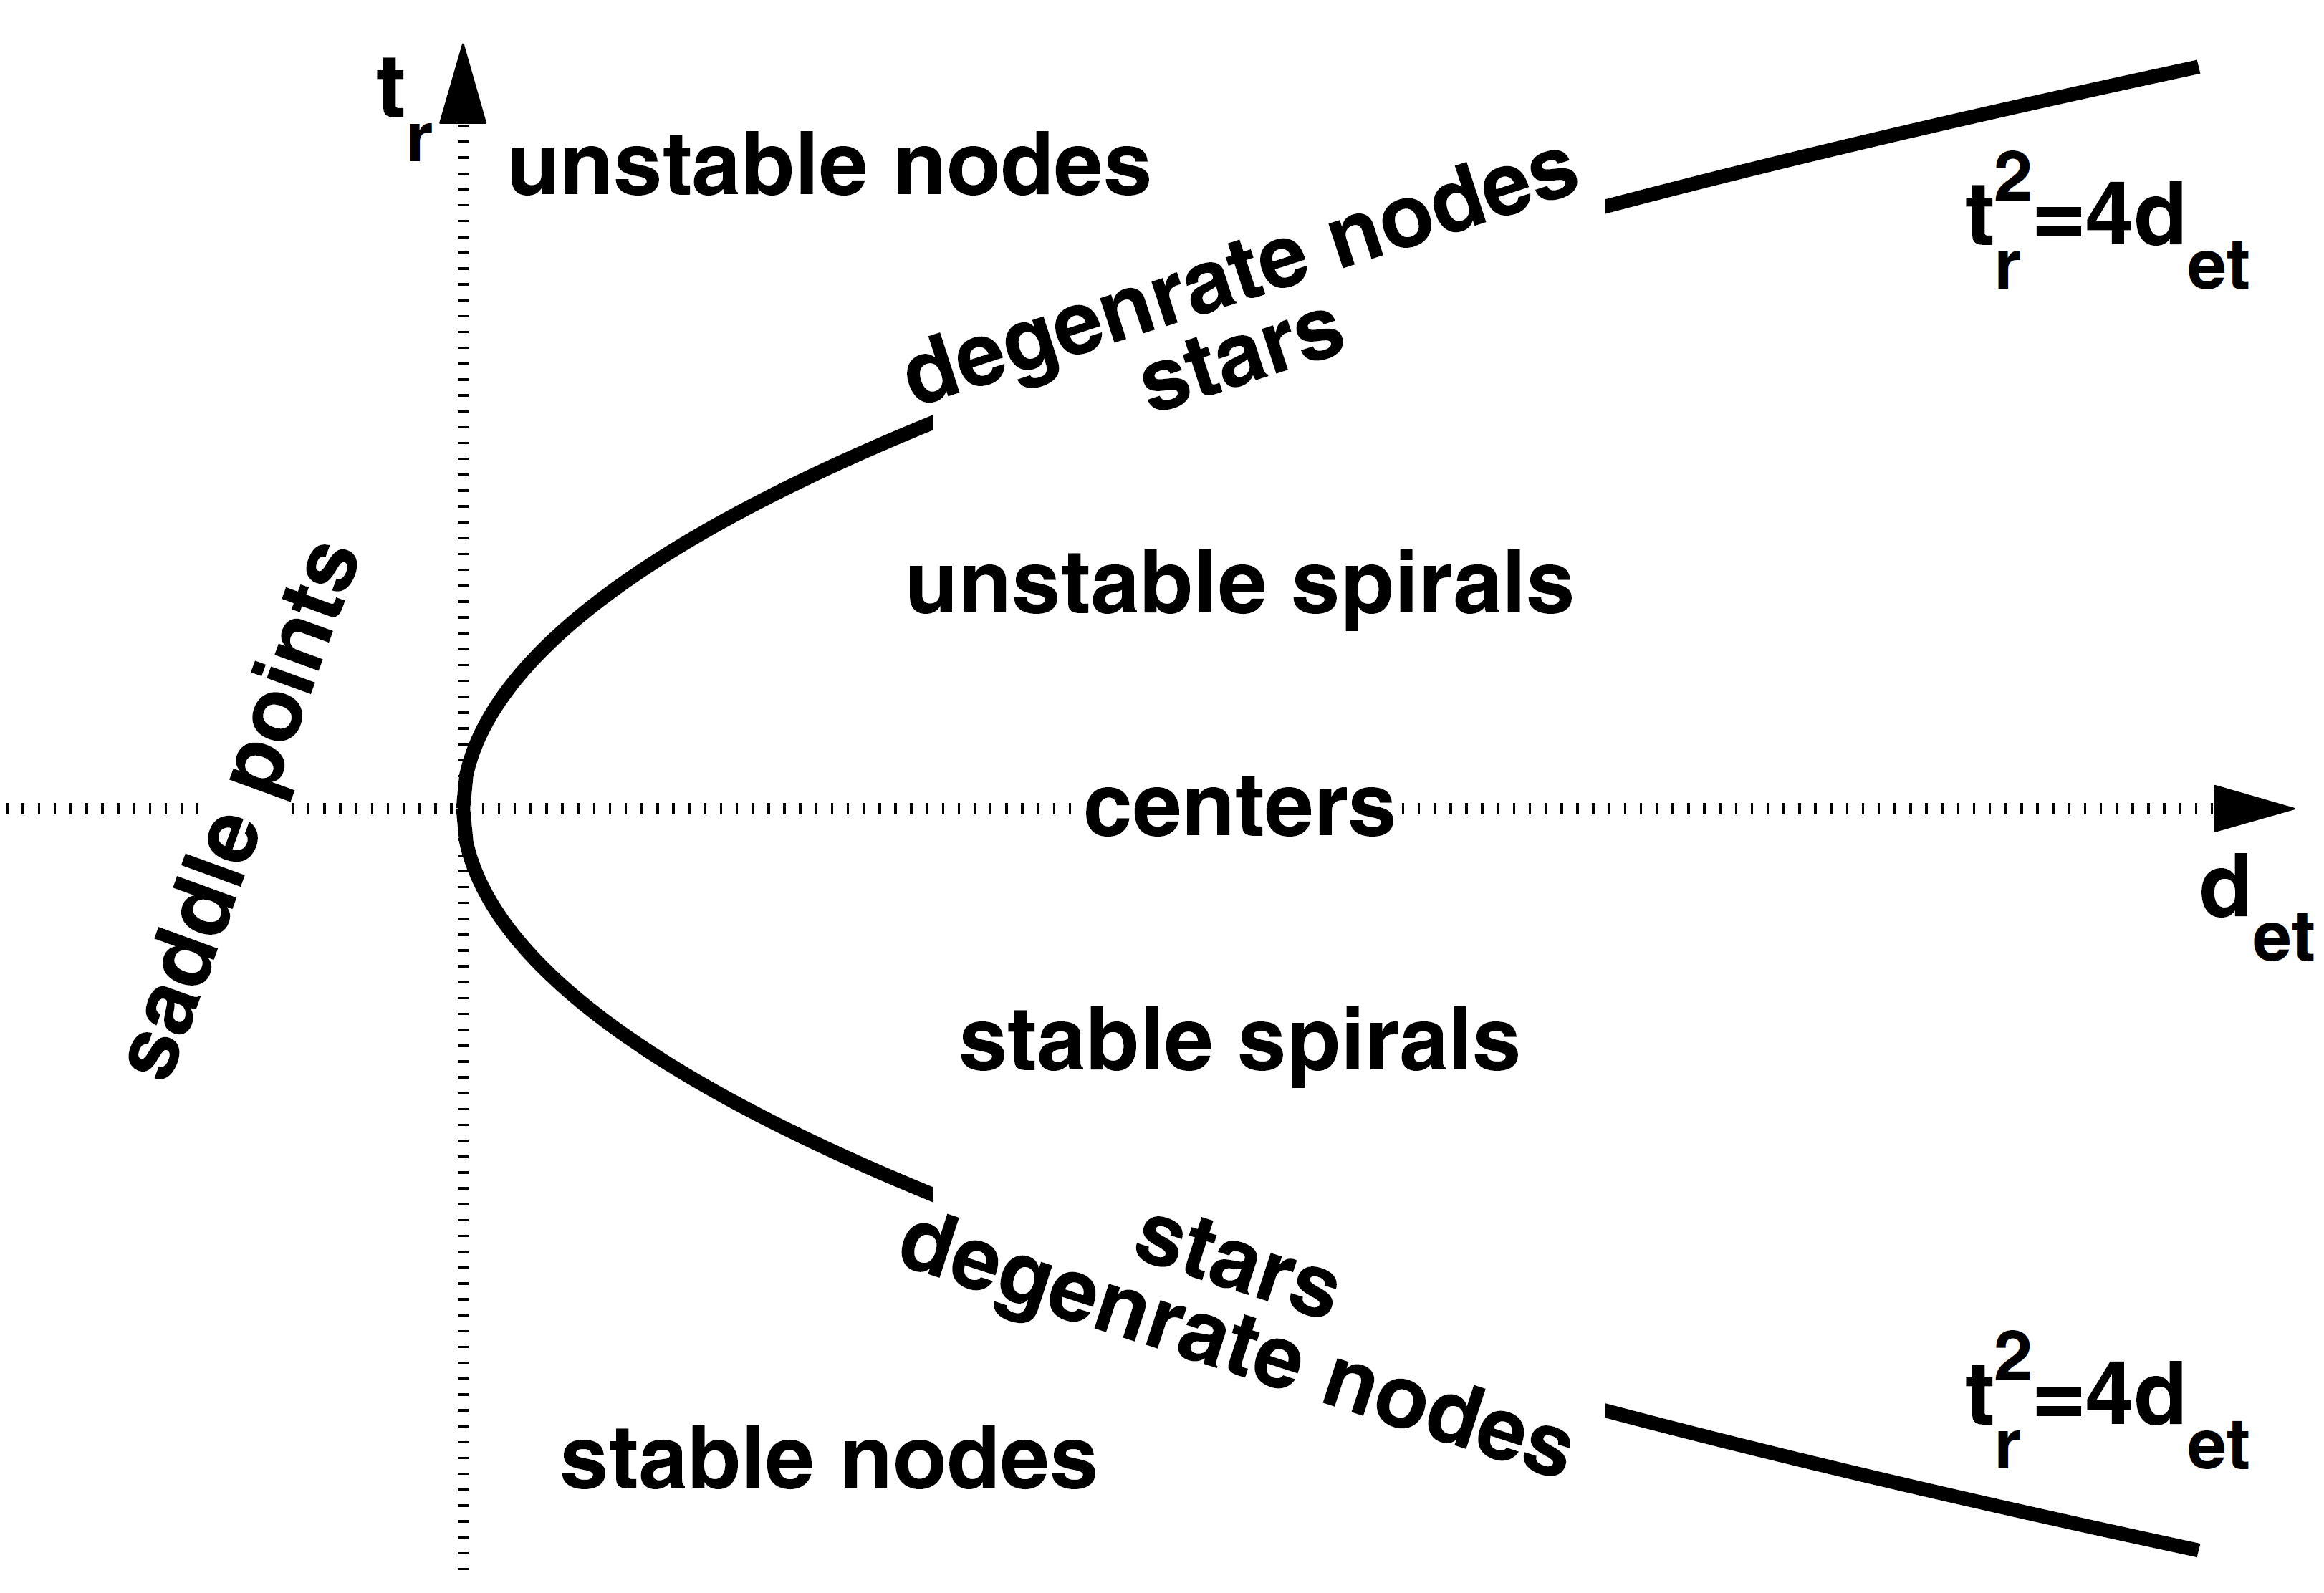
\includegraphics[width=0.5\linewidth]{sumls.png}
	\caption{Classification diagram for two-dimensional linear systems in terms of the trace $t_r$ and determinant $d_{et}$ of the linear matrix.}
	\label{fig:sumls}
\end{figure}
\subsection{Stability}
\subsubsection*{Attracting}
We say that $\mathbf{\tilde{x}}$ is \emph{attracting} if there is a $\delta>0$ such that $\displaystyle\lim_{t\rightarrow\infty}\mathbf{x}(t)=\mathbf{\tilde{x}}$ whenever $\|\mathbf{x}(0)-\mathbf{\tilde{x}}\|<\delta$.\\
Any trajectory that starts within a distance $\delta$ of $\mathbf{\tilde{x}}$ is guaranteed to converge to $\mathbf{\tilde{x}}$ eventually.\\
If $\mathbf{\tilde{x}}$ attracts all trajectories in the phase plane it is called {\textbf{globally attracting}}.
\subsubsection*{Lyapunov Stable}
We say that $\mathbf{\tilde{x}}$ is \emph{Lyapunov stable} if for each $\epsilon>0$, there is a $\delta>0$ such that $\|\mathbf{x}(0)-\mathbf{\tilde{x}}\|<\epsilon$ whenever $t\geq0$ and $\|\mathbf{x}(0)-\mathbf{\tilde{x}}\|<\delta$.\\
Lyapunov stability requires that nearby trajectories remain close for
all time.\\
Trajectories that start within $\delta$ of $\mathbf{\tilde{x}}$ remain within $\epsilon$ of $\mathbf{\tilde{x}}$ for all positive time.
\subsubsection*{Asymptotically stable}
$\mathbf{\tilde{x}}$ is \emph{asymptotically stable} if it is both attracting and Lyapunov stable.
\subsubsection*{Neutrally stable}
When a fixed point is Lyapunov stable but not attracting, it is called \emph{neutrally stable}.\\
Figure (\ref{fig:cnls}d) shows that a fixed point can be Lyapunov stable but not attracting.\\\\
It’s possible for a fixed point to be attracting but not Lyapunov stable. \\
Consider the system
\begin{equation}
	\dot{\theta}=1-\cos\theta
\end{equation}
\begin{theorem}[\textbf{The Lyapunov Stability Theorem}]{\label{thm:lst}}
	Consider a system $\mathbf{\dot{x}}=\mathbf{f(x)}$ with a fixed point at $\mathbf{\tilde{x}}$.
	Suppose that we can find a Lyapunov function, i.e., a continuously differentiable, real-valued function $V(x)$ (See Section (\ref{sec:pf2d})) with the following properties:
	\begin{itemize}
		\item $V(\mathbf{\tilde{x}})=0$
		\item $V(\mathbf{x})>0$ for all $\mathbf{x\neq\tilde{x}}$. (We say that $V$ is \emph{positive definite}.)
	\end{itemize}
	\begin{enumerate}
	\item if $\dot{V}\leq0$ for all $\mathbf{x}$, then $\mathbf{\tilde{x}}$ is \emph{stable};
	\item if $\dot{V}<0$ for all $\mathbf{x}$, then $\mathbf{\tilde{x}}$ is \emph{asymptotically} \emph{stable};
	\item if $\dot{V}>0$ for all $\mathbf{x}$, then $\mathbf{\tilde{x}}$ is \emph{unstable};
	\end{enumerate}
\end{theorem}
\subsubsection*{Basin of Attraction}
\begin{wrapfigure}{r}{0.3\linewidth}
	\centering
	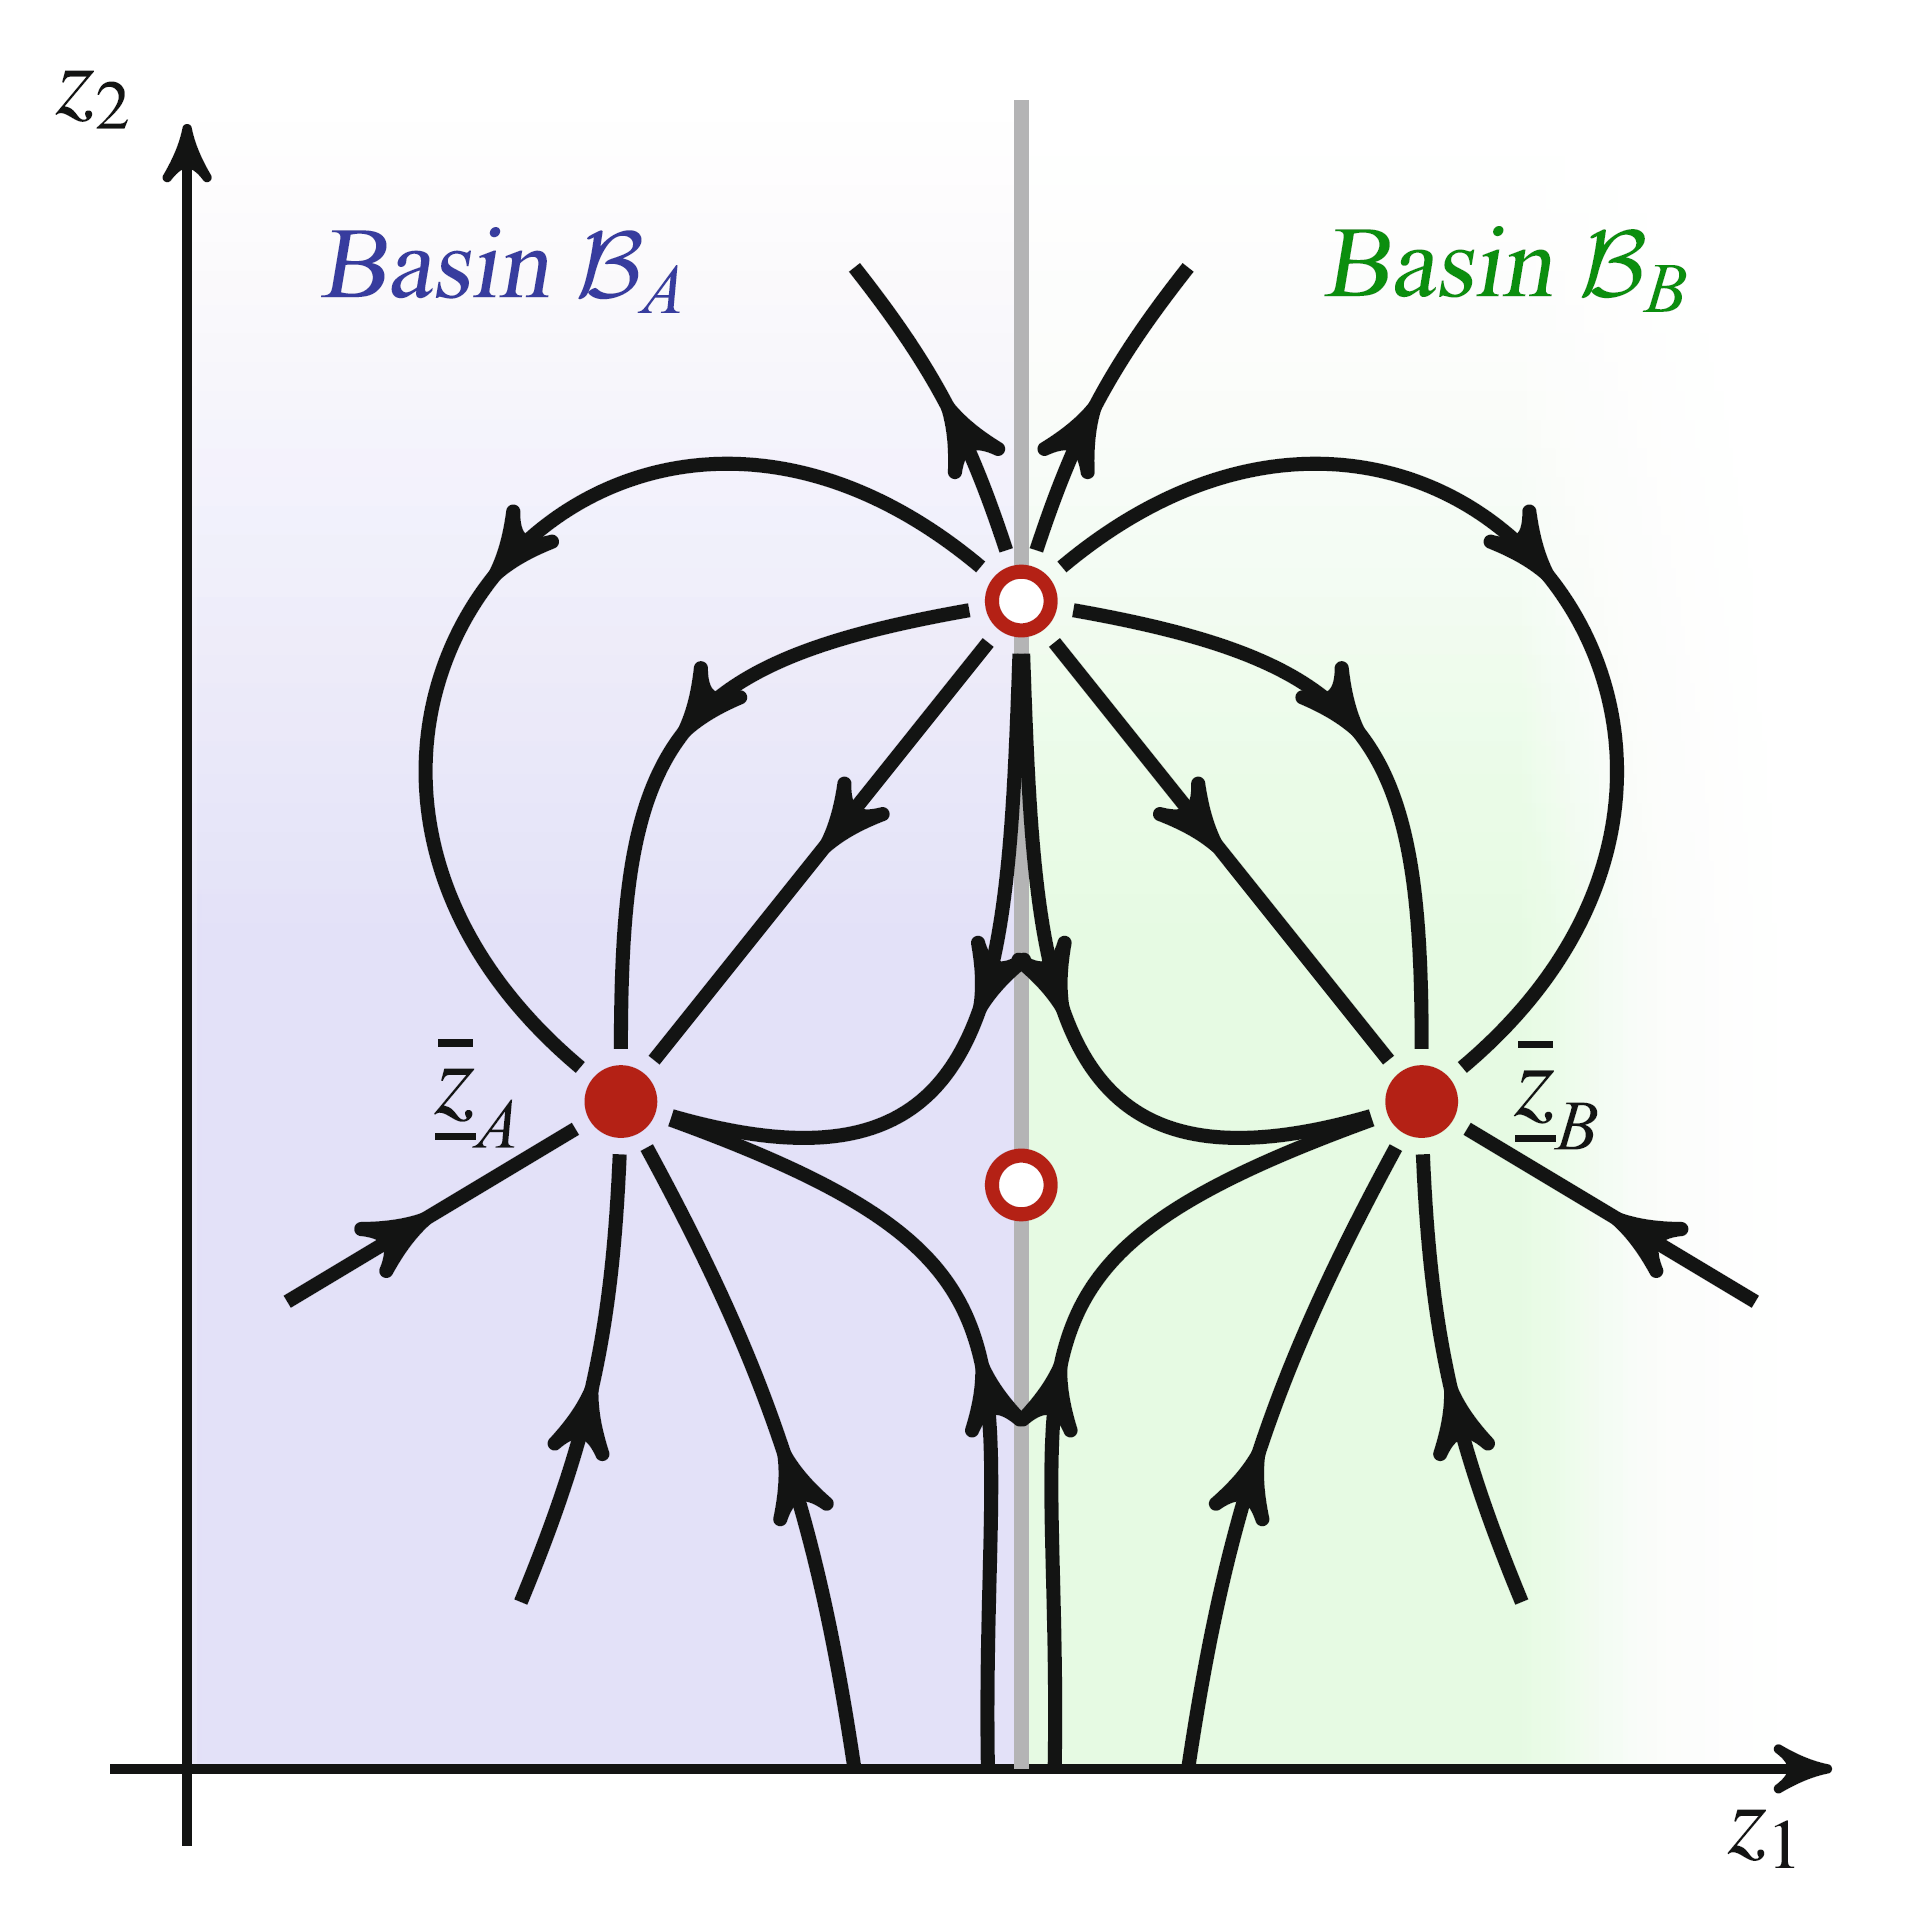
\includegraphics[width=\linewidth]{boa.png}
\end{wrapfigure}
A \emph{Basin of Attraction} describes that subset of the state space, such that initializing
the dynamics anywhere within the basin leads to convergence to a single
stable fixed point.
Thus all points $z$ in basin $\mathcal{B}_i$ converge to stable fixed point $\tilde{z}_i$.
\begin{equation}
	\mathcal{B}_i=\left\{z(0)\ \text{such that} \lim_{t\rightarrow\infty} z(t)=\tilde{z}_i \right\}
\end{equation}
\subsection{The Harmonic Oscillator}
\begin{equation}{\label{eq:tho}}
	\ddot{x}+\underbrace{\frac{\tilde{\gamma}}{m}}_{=2\gamma}\dot{x}+\underbrace{\frac{k}{m}}_{=\omega^2}x=0
\end{equation}
\subsubsection{Undamped Harmonic Oscillator}
If the damping constant vanishes, $\gamma=0$, (\ref{eq:tho}) simplifies to
\begin{equation}{\label{eq:bde2d}}
	\ddot{x}+\omega^2 x=0 
\end{equation}
The general solution of (\ref{eq:bde2d}) is given by
\begin{equation}
	x(t)=a\cos\omega t+b\sin\omega t
\end{equation}
In contrast to the first order systems we have dealt with so far, this general solution has not one but two free parameters, $a$ and $b$, that need to be determined from initial conditions.
\subsubsection{Damped Harmonic Oscillator}
\begin{equation}
	\ddot{x}+2\gamma\dot{x}+\omega^2x=0\quad\rightarrow\quad
	\begin{cases}
		\dot{x}=y\\
		\dot{y}=-\omega^2x-2\gamma y
	\end{cases}
\end{equation}
\begin{equation}
	\begin{pmatrix}
		\dot{x}\\\dot{y}
	\end{pmatrix}=
	\begin{pmatrix}
		0&1\\-\omega^2&-2\gamma
	\end{pmatrix}
	\begin{pmatrix}
		x\\y
	\end{pmatrix}
	\quad\rightarrow\quad
	\mathbf{\dot{x}}=A\mathbf{x}
\end{equation}
The eigenvectors are found from the relation
\begin{equation}
	A\mathbf{v}=\lambda\mathbf{v}\quad\rightarrow\quad
	\begin{pmatrix}
		0&1\\-\omega^2&-2\gamma
	\end{pmatrix}
	\begin{pmatrix}
		v_x\\v_y
	\end{pmatrix}=\lambda
	\begin{pmatrix}
		v_x\\v_y
	\end{pmatrix}
\end{equation}
\begin{equation}{\label{eq:dhos}}
	\rightarrow\quad\lambda_{1,2}=\left\{-\gamma\pm\sqrt{\gamma^2-\omega^2}\right\}
\end{equation}
By setting $v_x =1$, it is evident that oscillations can only occur if the eigenvalues have nonvanishing imaginary parts.
This means that the discriminant $\gamma^2-\omega^2$ in (\ref{eq:dhos}) must be smaller than zero.\\
Let $\gamma^2-\omega^2=-\Omega^2$ and $c=a+ib$.\\ 
The general solution  of (\ref{eq:tho}) is given by
\begin{equation}{\label{eq:gsho}}
	\begin{pmatrix}
		x(t)\\y(t)
	\end{pmatrix}=
	e^{-\gamma t}\left\{ce^{i\Omega t}
	\begin{pmatrix}
		1\\-\gamma+i\Omega
	\end{pmatrix}
	c^\ast e^{-i\Omega t}
	\begin{pmatrix}
		1\\-\gamma-i\Omega
	\end{pmatrix}\right\}
\end{equation}
which simplifies to 
\begin{equation}
	x(t)=e^{-\gamma t}\{a\cos\Omega t+b\sin\Omega t\}
\end{equation}
\begin{figure}[h!]
	\centering
	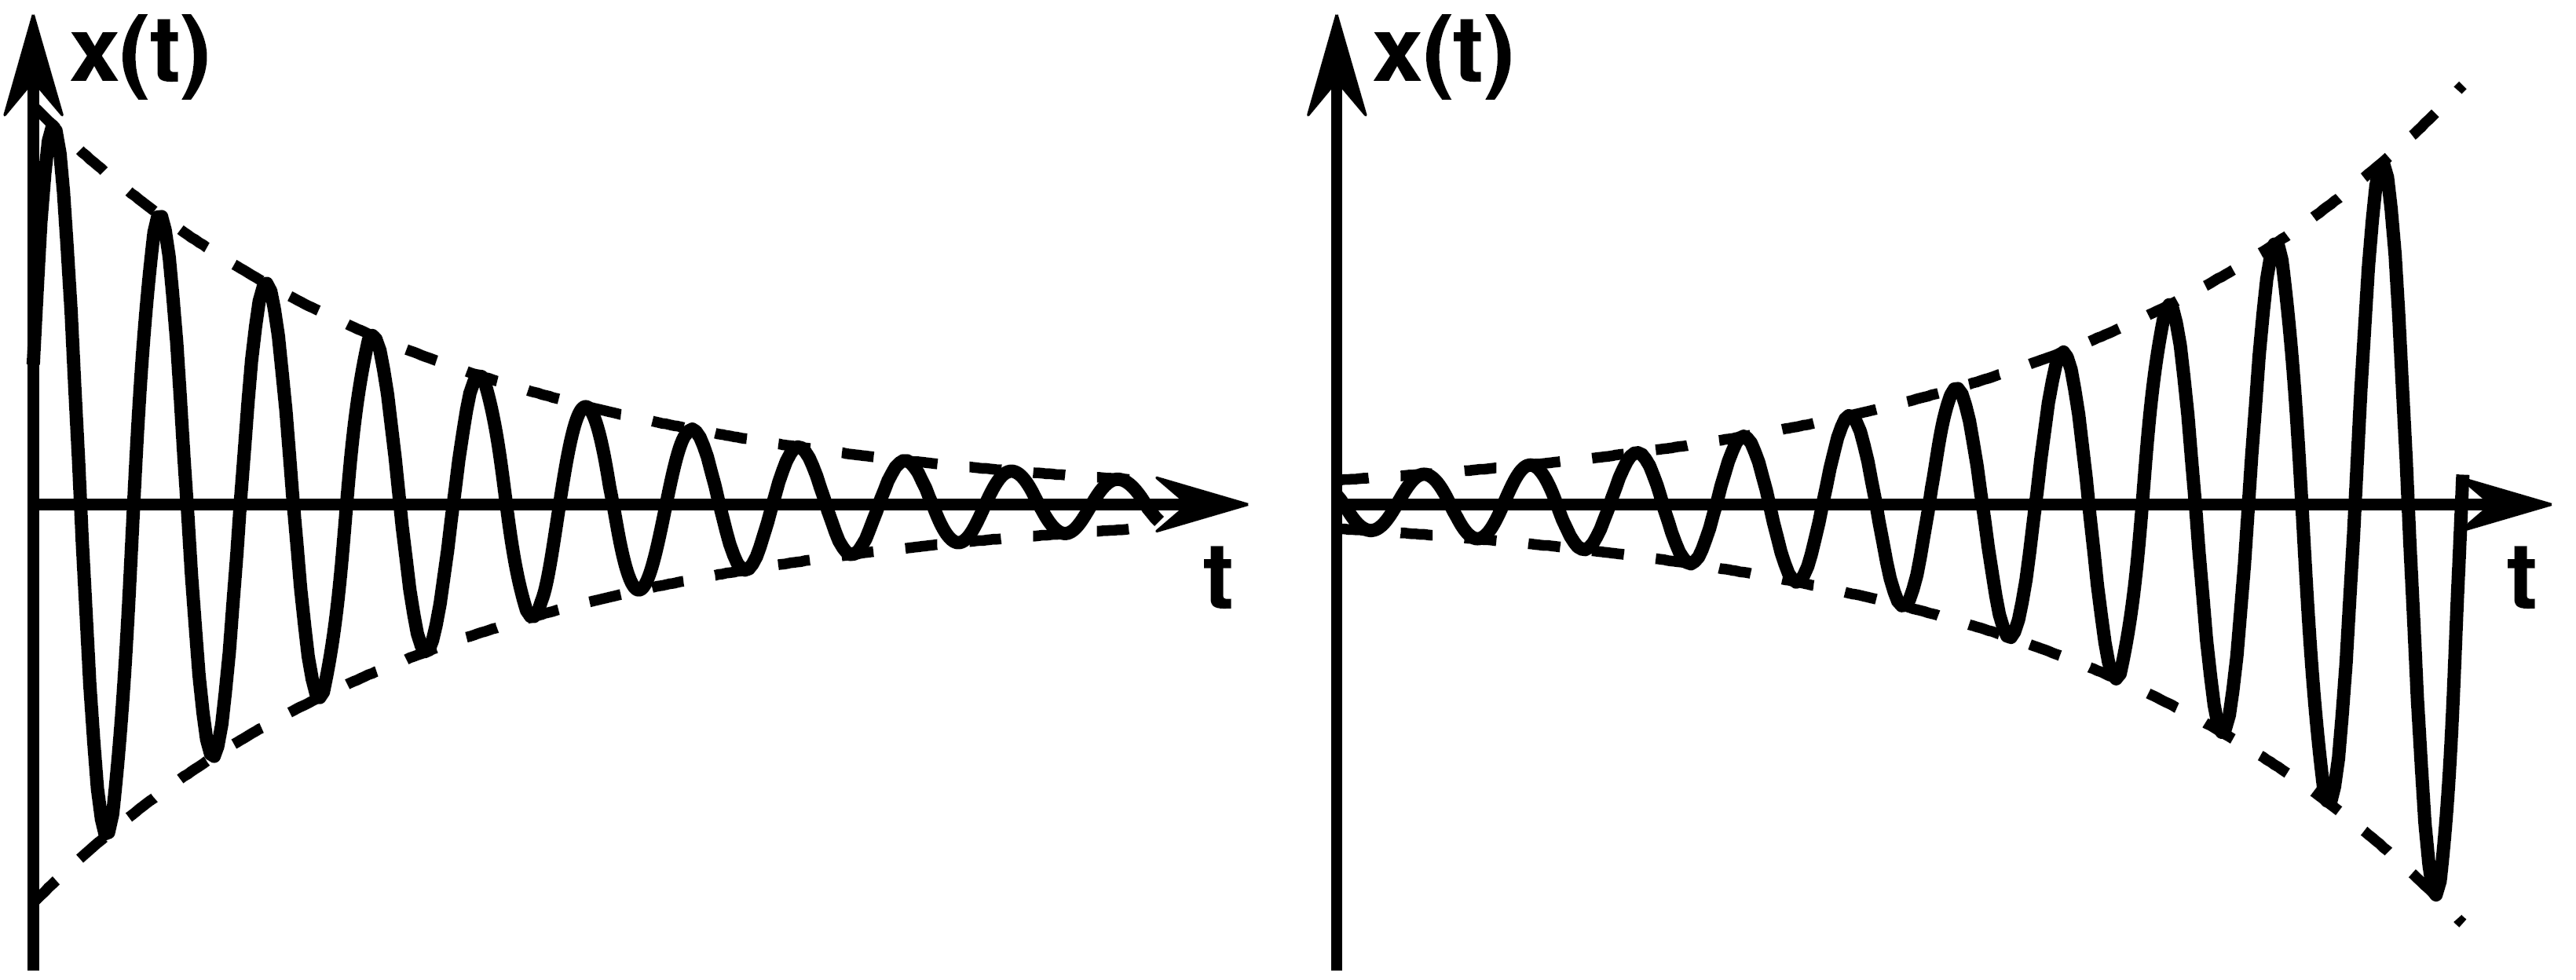
\includegraphics[width=0.5\linewidth]{dhs.png}
	\caption{Examples for damped harmonic oscillations for the case of positive damping $\gamma>0$ (left) and negative damping $\gamma>0$ (right).}
	\label{fig:dhs}
\end{figure}
If the damping constant $\gamma$ is greater than the angular velocity $\omega$ both eigenvalues are real numbers and the system does not oscillate. In this case equation (\ref{eq:gsho}) simplifies to 
\begin{equation}
	\begin{pmatrix}
		x(t)\\y(t)
	\end{pmatrix}=
	c_1e^{\lambda_1t}
	\begin{pmatrix}
		1\\\lambda_1
	\end{pmatrix}+
	c_2e^{\lambda_2t}
	\begin{pmatrix}
		1\\\lambda_2
	\end{pmatrix}\quad
	c_1,c_2\in\mathbb{R}
\end{equation}
which gives
\begin{equation}
	x(t)=c_1e^{\lambda_1t}+c_2e^{\lambda_2t}
\end{equation}
The solution is a superposition of two exponentials.